  \section[Convergent Medical Terminology (CMT)]{CMT}
  \label{sec:cmt}

  \initial{C}onvergent Medical Terminology (CMT) is a set of clinician and patient friendly\
  terminology, linked to US and international interoperability standards, and\
  related vocabulary development tools and utilities. Developed by Kaiser\-
  Permananente over many years for use within its health-IT systems, CMT now\
  includes more than 75,000 concepts. CMT is a core component Kaiser Permanente's\
  comprehensive electronic health record \emph{KP HealthConnect\textsuperscript\textregistered}.\\

  \begin{figure}[ht!]
    \centering
    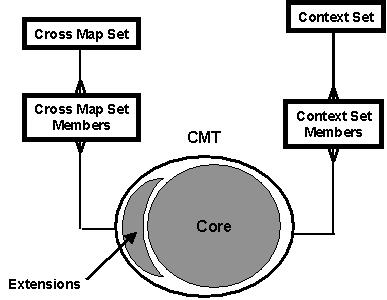
\includegraphics[scale=0.75]{CMT.jpg}
    \caption{High-level graphical description\
    of CMT}\citep[Fig.~1]{dolin_kaiser_2004}
    \label{fig:cmt}
  \end{figure}  

  \noindent In September 2010 Kaiser Permanente, the International Health\
  Terminology Standards Development Organisation (IHTSDO) and the US\
  Department of Health and Human Services jointly announced Kaiser Permanente's\
  donation of their CMT content and related tooling to the IHTSDO. The donation\
  consists of terminology content already developed, a set of tools to\
  help create and manage terminology and processes to control the quality of\
  terminology that is developed. CMT also includes mappings to classifications\
  and standard vocabularies including SNOMED CT\textsuperscript{\ref{sec:snomedct}}.\\
  
  \noindent A high-level graphical depiction of CMT\
  is shown in Figure~\ref{fig:cmt}. CMT is built upon\
  industry standard terminologies. SNOMED CT\textsuperscript{\ref{sec:snomedct}},\
  laboratory LOINC\textsuperscript{\ref{sec:loinc}} and First DataBank\textsuperscript{\ref{sec:fdb}} drug\
  terminology form the core of CMT. Core terminologies are integrated into a\
  single poly-hierarchically structured knowledge base. A classifier organizes\
  the CMT concepts into a poly-hierarchy, based on their definitions.\
  The act of classifying helps identify synonymous concepts, and maintains quality\
  and consistency across the some 400,000 concepts.\\
  
  \noindent Applications can directly access CMT via a provided interface and/or\
  CMT can provide applications with cross map sets and context sets, both of which\
  are patterned after the SNOMED CT\textsuperscript{\ref{sec:snomedct}} model.\
  Cross map sets are used to store mappings between CMT concepts and other coding schemes.\
  Context sets are CMT subsets used within a particular context. Contexts\
  can include a particular drop-down list or vocabulary table in an application,\
  a field in an HL7\textsuperscript{\ref{sec:fhir}} message, or any other CMT\
  subset needed within the organization.\\
  
  \noindent CMT is currently distributed within the UMLS Metathesauras\
  (\url{http://www.nlm.nih.gov/research/umls/knowledge_sources/metathesaurus/index.html}).
